\documentclass{standalone}
\usepackage{tikz}
\usetikzlibrary{angles, quotes}

\begin{document}
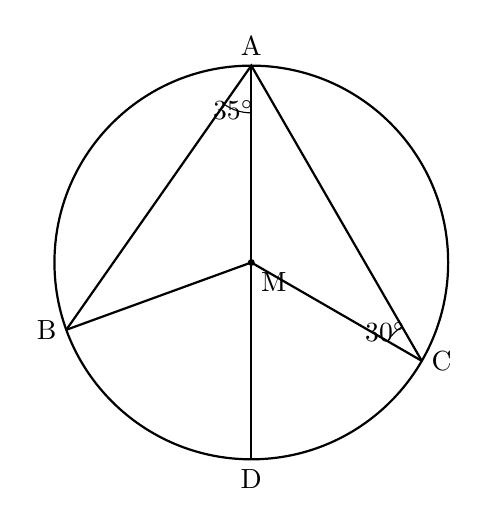
\begin{tikzpicture}[scale=2.5]
    % কেন্দ্র এবং বৃত্ত অঙ্কন
    \coordinate (M) at (0, 0);
    \draw[thick] (M) circle (1);
    
    % বিন্দুর স্থানাঙ্ক নির্ধারণ (AD ব্যাস এবং নির্দিষ্ট কোণ অনুযায়ী)
    \coordinate (A) at (90:1);
    \coordinate (D) at (270:1);
    \coordinate (B) at (200:1); % কেন্দ্রস্থ কোণ AMB = 110 ডিগ্রি হলে বৃত্তস্থ BAM = 35
    \coordinate (C) at (330:1); % কেন্দ্রস্থ কোণ AMC = 120 ডিগ্রি হলে বৃত্তস্থ MAC/ACM = 30
    
    % রেখা এবং ব্যাসার্ধ অঙ্কন
    \draw[thick] (A) -- (D); % ব্যাস AD
    \draw[thick] (B) -- (A) -- (C); % জ্যা AB এবং AC
    \draw[thick] (B) -- (M) -- (C); % ব্যাসার্ধ MB এবং MC
    \draw[thick] (M) -- (A); % ব্যাসার্ধ MA
    
    % লেবেল প্রদান
    \node[above] at (A) {A};
    \node[below] at (D) {D};
    \node[left] at (B) {B};
    \node[right] at (C) {C};
    \node[below right] at (M) {M};
    \fill (M) circle (0.5pt); % কেন্দ্রবিন্দু
    
    % কোণ চিহ্নিতকরণ (Angle Radius সহ)
    % vertex A তে 35 ডিগ্রি
    \pic [draw, angle radius=0.6cm, "$35^{\circ}$" {shift={(-0.12, -0.22)}}] {angle = B--A--M};
    % vertex C তে 30 ডিগ্রি (আপনার সংশোধিত তথ্য অনুযায়ী)
    \pic [draw, angle radius=0.5cm, "$30^{\circ}$" {shift={(-0.25, 0.15)}}] {angle = A--C--M};
\end{tikzpicture}
\end{document}